\chapter{Risultati Sperimentali}
\label{chap:risultati}

Questo capitolo presenta i risultati ottenuti con lo split group-aware su UCF-101. Tutti i valori di accuratezza riportati come ``Test'' si riferiscono al test set ufficiale; quelli come ``Val'' si riferiscono alla porzione di validation estratta dal training set con split group-aware.

\section{Modelli di Riferimento}

\begin{table}[H]
\centering
\caption{Performance dei modelli di riferimento sul test set ufficiale.}
\label{tab:baselines}
\begin{tabular}{lcccc}
\toprule
\textbf{Modello} & \textbf{Val Top-1} & \textbf{Test Top-1} & \textbf{Test Top-5} & \textbf{Size (MB)} \\
\midrule
Teacher (3D ResNet-50) & 92.36\% & 88.82\% & 98.18\% & $\sim$128 \\
Baseline (MobileNet3D)  & 59.18\% & 59.48\% & 82.77\% & $\sim$9.5 \\
\bottomrule
\end{tabular}
\end{table}

Il \textbf{gap} tra teacher e baseline è di circa \textbf{29.3 punti percentuali} in Top-1, confermando l'esistenza di un significativo \textit{capacity gap} tra le due architetture. Questo gap è la motivazione fondamentale per la Knowledge Distillation: trasferire allo student parte della conoscenza strutturale del teacher che non emerge dal solo addestramento con hard labels.

\section{Knowledge Distillation: Risultato Principale}

L'esperimento principale di KD utilizza temperatura $T = 8$ e $\alpha = 0.7$:

\begin{table}[H]
\centering
\caption{Confronto Baseline vs Knowledge Distillation ($T=8$, $\alpha=0.7$).}
\label{tab:kd_main}
\begin{tabular}{lcccc}
\toprule
\textbf{Modello} & \textbf{Val Top-1} & \textbf{Test Top-1} & \textbf{Test Top-5} & \textbf{$\Delta$ vs Baseline} \\
\midrule
Baseline            & 59.18\% & 59.48\% & 82.77\% & --- \\
KD ($T=8$)          & 64.57\% & 64.31\% & 87.68\% & \textbf{+4.83\%} \\
\bottomrule
\end{tabular}
\end{table}

La Knowledge Distillation produce un miglioramento significativo di \textbf{+4.83 punti percentuali} in Test Top-1 e +4.91\% in Top-5, senza alcuna modifica all'architettura del modello. Lo student distillato raggiunge il 64.31\% mantenendo la stessa dimensione di 9.5~MB e la latenza di $\sim$1.8~ms.

\begin{figure}[H]
    \centering
    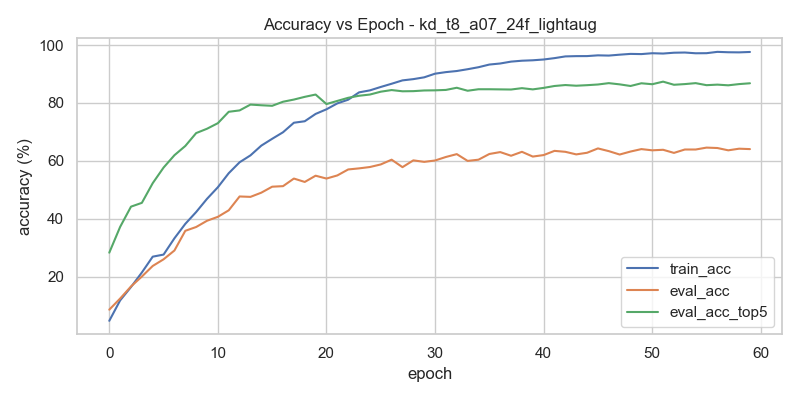
\includegraphics[width=0.8\textwidth]{parts/cap6_risultati/training_curves/kd_t8_a07_24f_lightaug_accuracy.png}
    \caption{Curve di accuracy per il training di KD con $T=8$, $\alpha=0.7$. Si noti il gap tipico tra training accuracy ($\sim$98\%) e validation accuracy ($\sim$64\%), indicativo della difficoltà del task con split group-aware.}
    \label{fig:kd_accuracy}
\end{figure}

\begin{figure}[H]
    \centering
    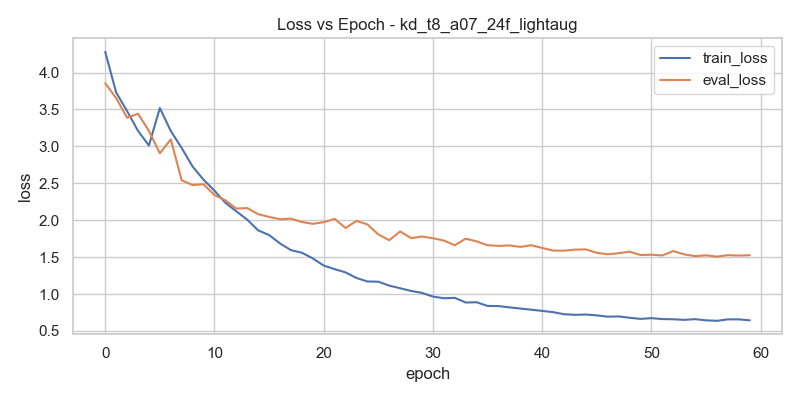
\includegraphics[width=0.8\textwidth]{parts/cap6_risultati/training_curves/kd_t8_a07_24f_lightaug_loss.png}
    \caption{Andamento della loss durante il training di KD ($T=8$).}
    \label{fig:kd_loss}
\end{figure}

\section{Temperature Scaling Ablation}
\label{sec:temp_sweep}

È stato condotto uno studio ablativo sistematico dell'effetto della temperatura sulle soft distributions del teacher:

\begin{table}[H]
\centering
\caption{Ablazione sulla temperatura con $\alpha = 0.7$ fisso.}
\label{tab:temp_ablation}
\begin{tabular}{ccccccc}
\toprule
\textbf{$T$} & \textbf{Best Val} & \textbf{Best Epoch} & \textbf{Train Acc} & \textbf{Test Top-1} & \textbf{Test Top-5} & \textbf{$\Delta$ vs BL} \\
\midrule
1  & 62.75\% & 60 & 98.44\% & 62.91\% & 85.59\% & +3.43\% \\
5  & 63.12\% & 57 & 95.87\% & 62.07\% & 87.02\% & +2.59\% \\
8  & 64.57\% & 56 & 97.59\% & 64.31\% & 87.68\% & +4.83\% \\
10 & 64.85\% & 60 & 98.28\% & 64.47\% & 87.44\% & +4.99\% \\
20 & 65.18\% & 59 & 99.05\% & \textbf{65.85\%} & \textbf{87.81\%} & \textbf{+6.37\%} \\
\bottomrule
\end{tabular}
\end{table}

\subsection{Analisi dei Risultati}

L'andamento mostra un chiaro trend crescente con la temperatura. La configurazione con $T = 20$ raggiunge la migliore Test Top-1 accuracy (\textbf{65.85\%}), con un miglioramento di \textbf{+6.37 punti percentuali} rispetto al baseline.

Questo risultato suggerisce che, per il gap di capacità significativo tra 3D ResNet-50 e MobileNet3D, temperature più alte che producono distribuzioni più uniformi risultano più efficaci. Con temperature basse ($T = 1$), le predizioni del teacher sono troppo ``peaky'' e lo student fatica a replicare la distribuzione inter-classe. Temperature alte ($T = 20$) ``smussano'' la distribuzione del teacher, esponendo relazioni tra classi che uno student limitato può meglio approssimare.

\begin{figure}[H]
    \centering
    
\includegraphics[width=0.9\textwidth]{parts/cap6_risultati/delta_accuracy_kd_vs_baseline.png}
    \caption{Delta di accuratezza (test) rispetto al baseline per ciascuna temperatura. Trend crescente con la temperatura, con picco a $T = 20$.}
    \label{fig:delta_temp}
\end{figure}

\section{Attention Transfer}
\label{sec:at_results}

L'Attention Transfer estende la KD con il trasferimento delle mappe di attenzione intermedie. Sono state testate due configurazioni:

\begin{table}[H]
\centering
\caption{Risultati dell'Attention Transfer (split group-aware). Le colonne $\beta_s$ e $\beta_t$ indicano i pesi delle componenti spaziale e temporale.}
\label{tab:at_results}
\begin{tabular}{lccccc}
\toprule
\textbf{Config} & $\beta_s$ & $\beta_t$ & \textbf{Val Top-1} & \textbf{Train Acc} \\
\midrule
KD ($T=8$, no AT)   & 0     & 0     & 64.57\% & 97.59\% \\
AT Simmetrico       & 0.05  & 0.05  & 58.25\% & 96.27\% \\
AT Temporal-Only    & 0     & 0.10  & 59.04\% & 95.87\% \\
\bottomrule
\end{tabular}
\end{table}

\subsection{Analisi del Risultato Negativo}

L'Attention Transfer non ha migliorato le prestazioni rispetto alla sola KD. Anzi, entrambe le configurazioni producono una \textbf{regressione} di 5--6 punti percentuali. Diverse ipotesi spiegano questo risultato:

\begin{enumerate}
    \item \textbf{Capacity gap spaziale}: il teacher utilizza convoluzioni standard 3D con $C \gg 1$ canali che interagiscono liberamente, producendo mappe di attenzione spaziale ricche e dettagliate. Il MobileNet3D utilizza convoluzioni depthwise separabili, dove ciascun canale è processato indipendentemente; questo limita intrinsecamente la capacità dello student di riprodurre le mappe spaziali del teacher.
    
    \item \textbf{Regularizzazione eccessiva}: il segnale AT spaziale può agire come un vincolo troppo restrittivo sulle feature intermedie, impedendo allo student di trovare soluzioni alternative compensatorie adatte alla sua architettura più limitata.
    
    \item \textbf{Dominanza del componente temporale}: l'AT puramente temporale ($\beta_s = 0$, $\beta_t = 0.1$) performa leggermente meglio del simmetrico, suggerendo che il componente spaziale è il principale responsabile della regressione.
\end{enumerate}

Questo risultato è coerente con la letteratura: il paper originale di Zagoruyko e Komodakis~\cite{zagoruyko2017paying} lavora con architetture della stessa famiglia (ResNet teacher $\rightarrow$ ResNet student), dove la similarità strutturale rende le mappe di attenzione più trasferibili.

\section{Born-Again Networks}
\label{sec:born_again}

Le Born-Again Networks tentano di migliorare lo student tramite self-distillation iterativa. Il migliore KD student ($T = 8$, $\alpha = 0.7$) diventa il teacher della Generazione~1, che a sua volta diventa teacher della Generazione~2, e così via.

\begin{table}[H]
\centering
\caption{Risultati Born-Again Networks (3 generazioni successive). Si noti il collasso progressivo delle prestazioni.}
\label{tab:born_again}
\begin{tabular}{lcccc}
\toprule
\textbf{Generazione} & \textbf{Teacher} & \textbf{Val Top-1} & \textbf{Test Top-1} & \textbf{$\Delta$ vs Gen0} \\
\midrule
Gen 0 (KD $T=8$) & ResNet-50 & 64.57\% & 64.31\% & --- \\
Gen 1              & Gen 0     & 60.78\% & 60.98\% & $-3.33$\% \\
Gen 2              & Gen 1     & 61.20\% & 60.43\% & $-3.88$\% \\
Gen 3              & Gen 2     & 59.98\% & 59.21\% & $-5.10$\% \\
\bottomrule
\end{tabular}
\end{table}

\subsection{Collasso Generazionale}

Il risultato mostra un chiaro \textbf{collasso generazionale}: ogni iterazione successiva produce prestazioni inferiori, anziché il miglioramento atteso dalla teoria~\cite{furlanello2018born}. Il collasso è progressivo: Gen~3 scende sotto il livello del baseline originale (59.21\% vs 59.48\%).

Le cause identificate:

\begin{enumerate}
    \item \textbf{Temperature non calibrata}: la temperatura $T = 2.5$ usata per la self-distillation era stata scelta per un teacher oracolo (ResNet-50 a $\sim$89\%). Un MobileNet3D a $\sim$64\% produce distribuzioni soft meno informative, e una temperatura troppo alta le rende ancora più piatte, diluendo il segnale utile.
    
    \item \textbf{Assenza di oracolo}: le Born-Again Networks presuppongono che il teacher della generazione $k$ sia almeno competente quanto quello della generazione $k-1$. Quando il teacher iniziale è già un modello limitato, il degrado della qualità del segnale si accumula.
    
    \item \textbf{Overfitting sugli artefatti}: il teacher non-oracolo commette errori sistematici che vengono amplificati e rinforzati nelle generazioni successive.
\end{enumerate}

\section{Visualizzazione t-SNE dello Spazio Latente}

La t-SNE è stata applicata alle embedding pre-classificatore per analizzare qualitativamente le rappresentazioni apprese. Per ciascuna visualizzazione, vengono selezionate 10 classi casuali e proiettate in 2D.

\begin{figure}[H]
    \centering
    
\includegraphics[width=\textwidth]{parts/cap6_risultati/tsne/tsne_comparison_4495.png}
    \caption{t-SNE a tre colonne: Teacher (ResNet-50), Baseline (MobileNet3D), e Student distillato (KD $T=8$). Il teacher mostra cluster compatti e ben separati; il baseline presenta sovrapposizione; lo student distillato mostra una struttura intermedia migliorata.}
    \label{fig:tsne_main}
\end{figure}

\begin{figure}[H]
    \centering
    
\includegraphics[width=\textwidth]{parts/cap6_risultati/tsne/tsne_teacher_baseline_at_comparison.png}
    \caption{t-SNE per i modelli con Attention Transfer: il pattern di clustering è simile a quello del baseline, confermando che l'AT non ha prodotto miglioramenti strutturali nelle rappresentazioni.}
    \label{fig:tsne_at}
\end{figure}

\begin{figure}[H]
    \centering
    
\includegraphics[width=\textwidth]{parts/cap6_risultati/tsne/tsne_born_again_final.png}
    \caption{t-SNE delle Born-Again Networks: la struttura non migliora nelle generazioni successive, coerentemente con il collasso osservato nelle metriche quantitative.}
    \label{fig:tsne_born}
\end{figure}

\section{Confusion Matrix}

Le confusion matrix normalizzate evidenziano le classi più confuse. Per leggibilità, vengono mostrate le Top-25 classi più problematiche.

\begin{figure}[H]
    \centering
    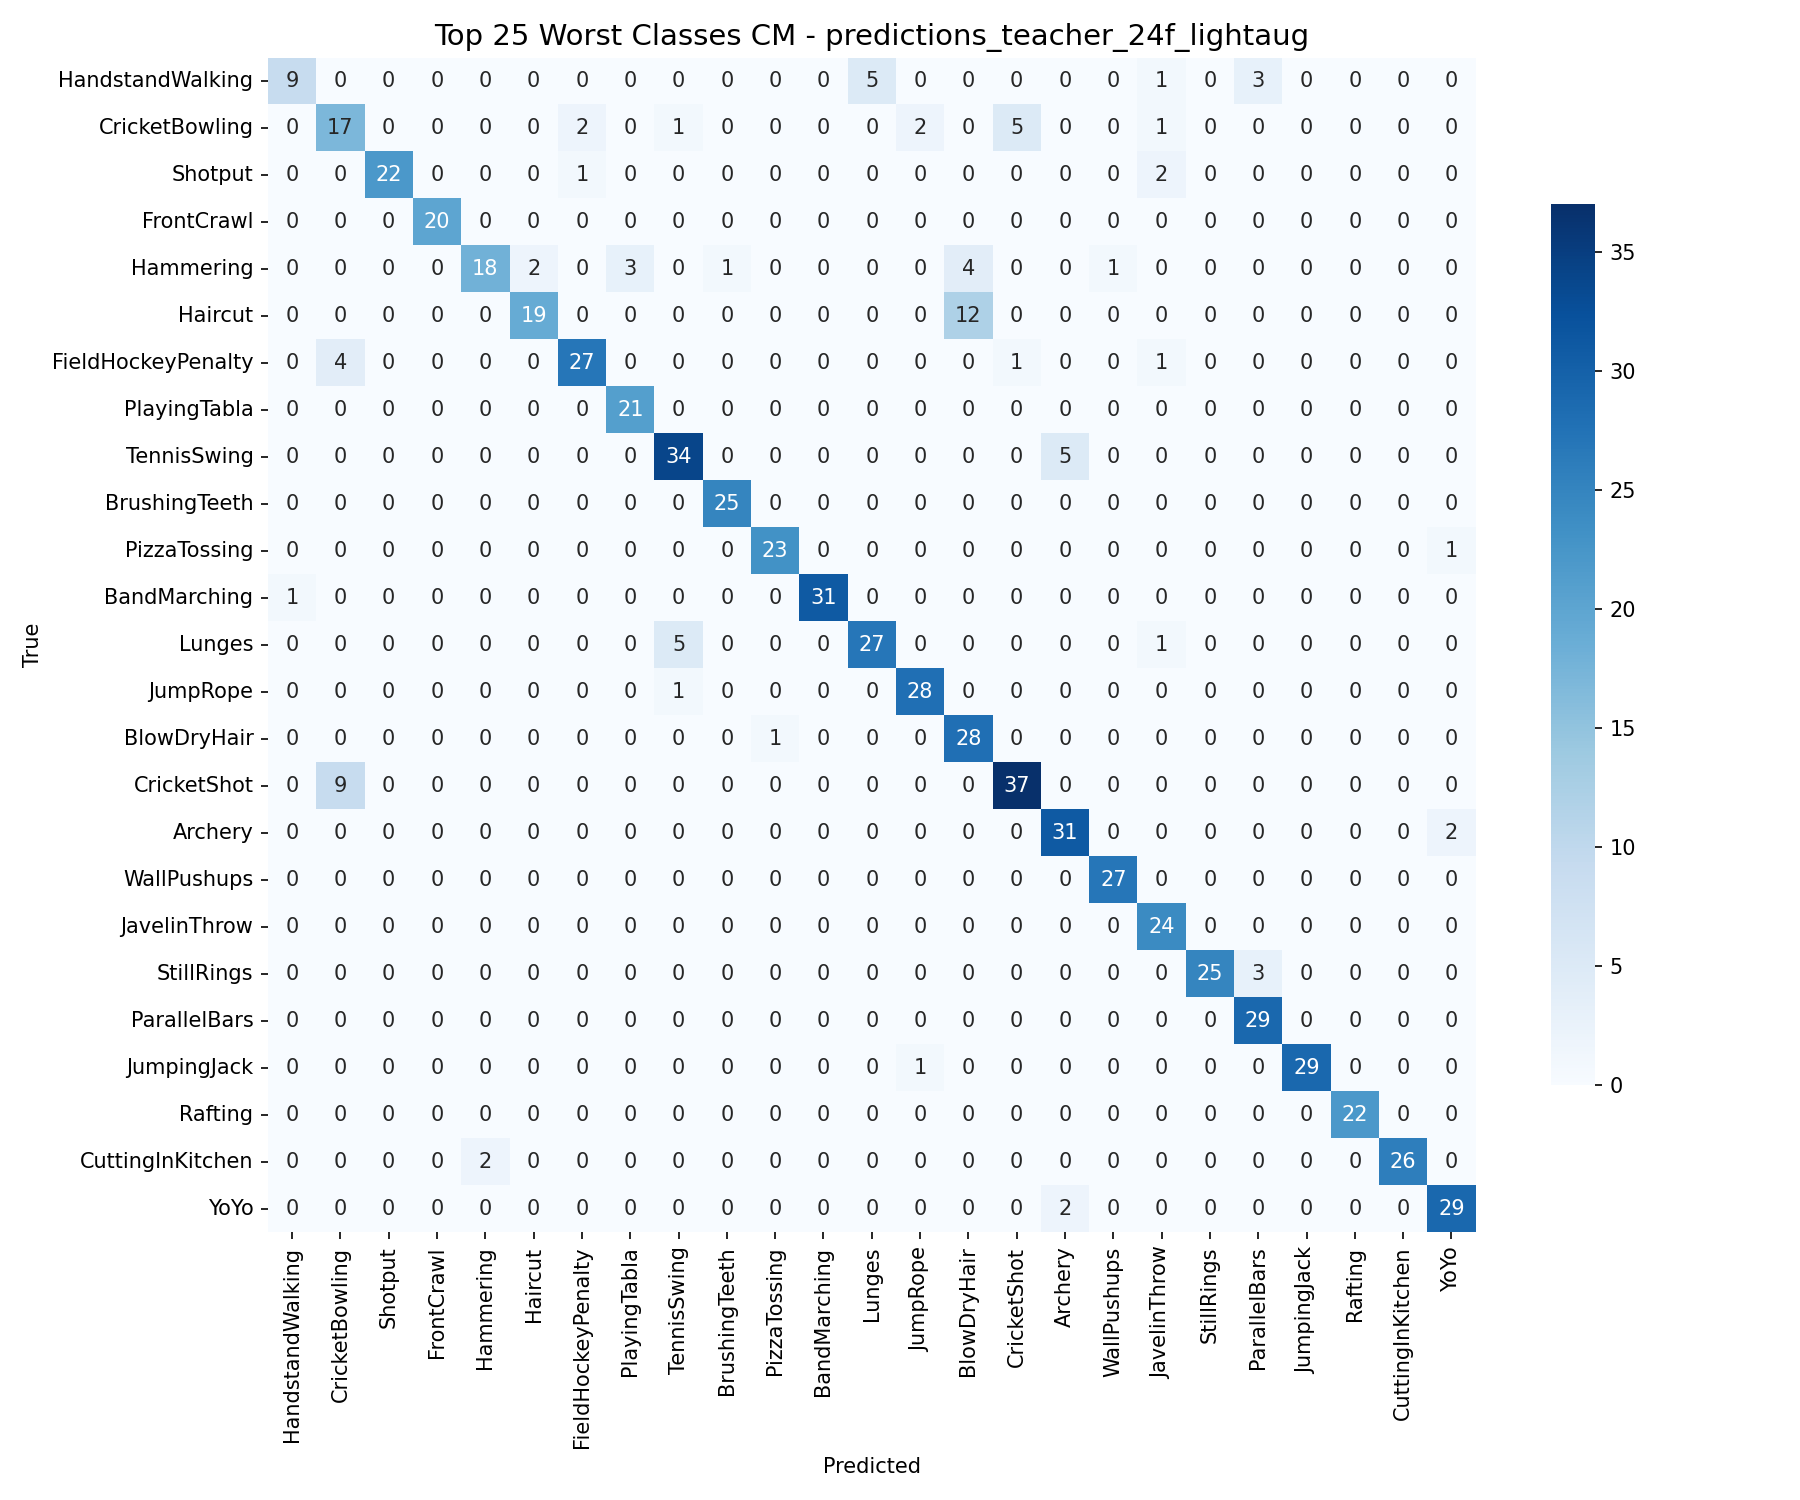
\includegraphics[width=0.85\textwidth]{parts/cap6_risultati/confusion_matrices/predictions_teacher_24f_lightaug_top25.png}
    \caption{Confusion matrix Top-25 del Teacher: errori concentrati su classi semanticamente ambigue.}
    \label{fig:cm_teacher}
\end{figure}

\begin{figure}[H]
    \centering
    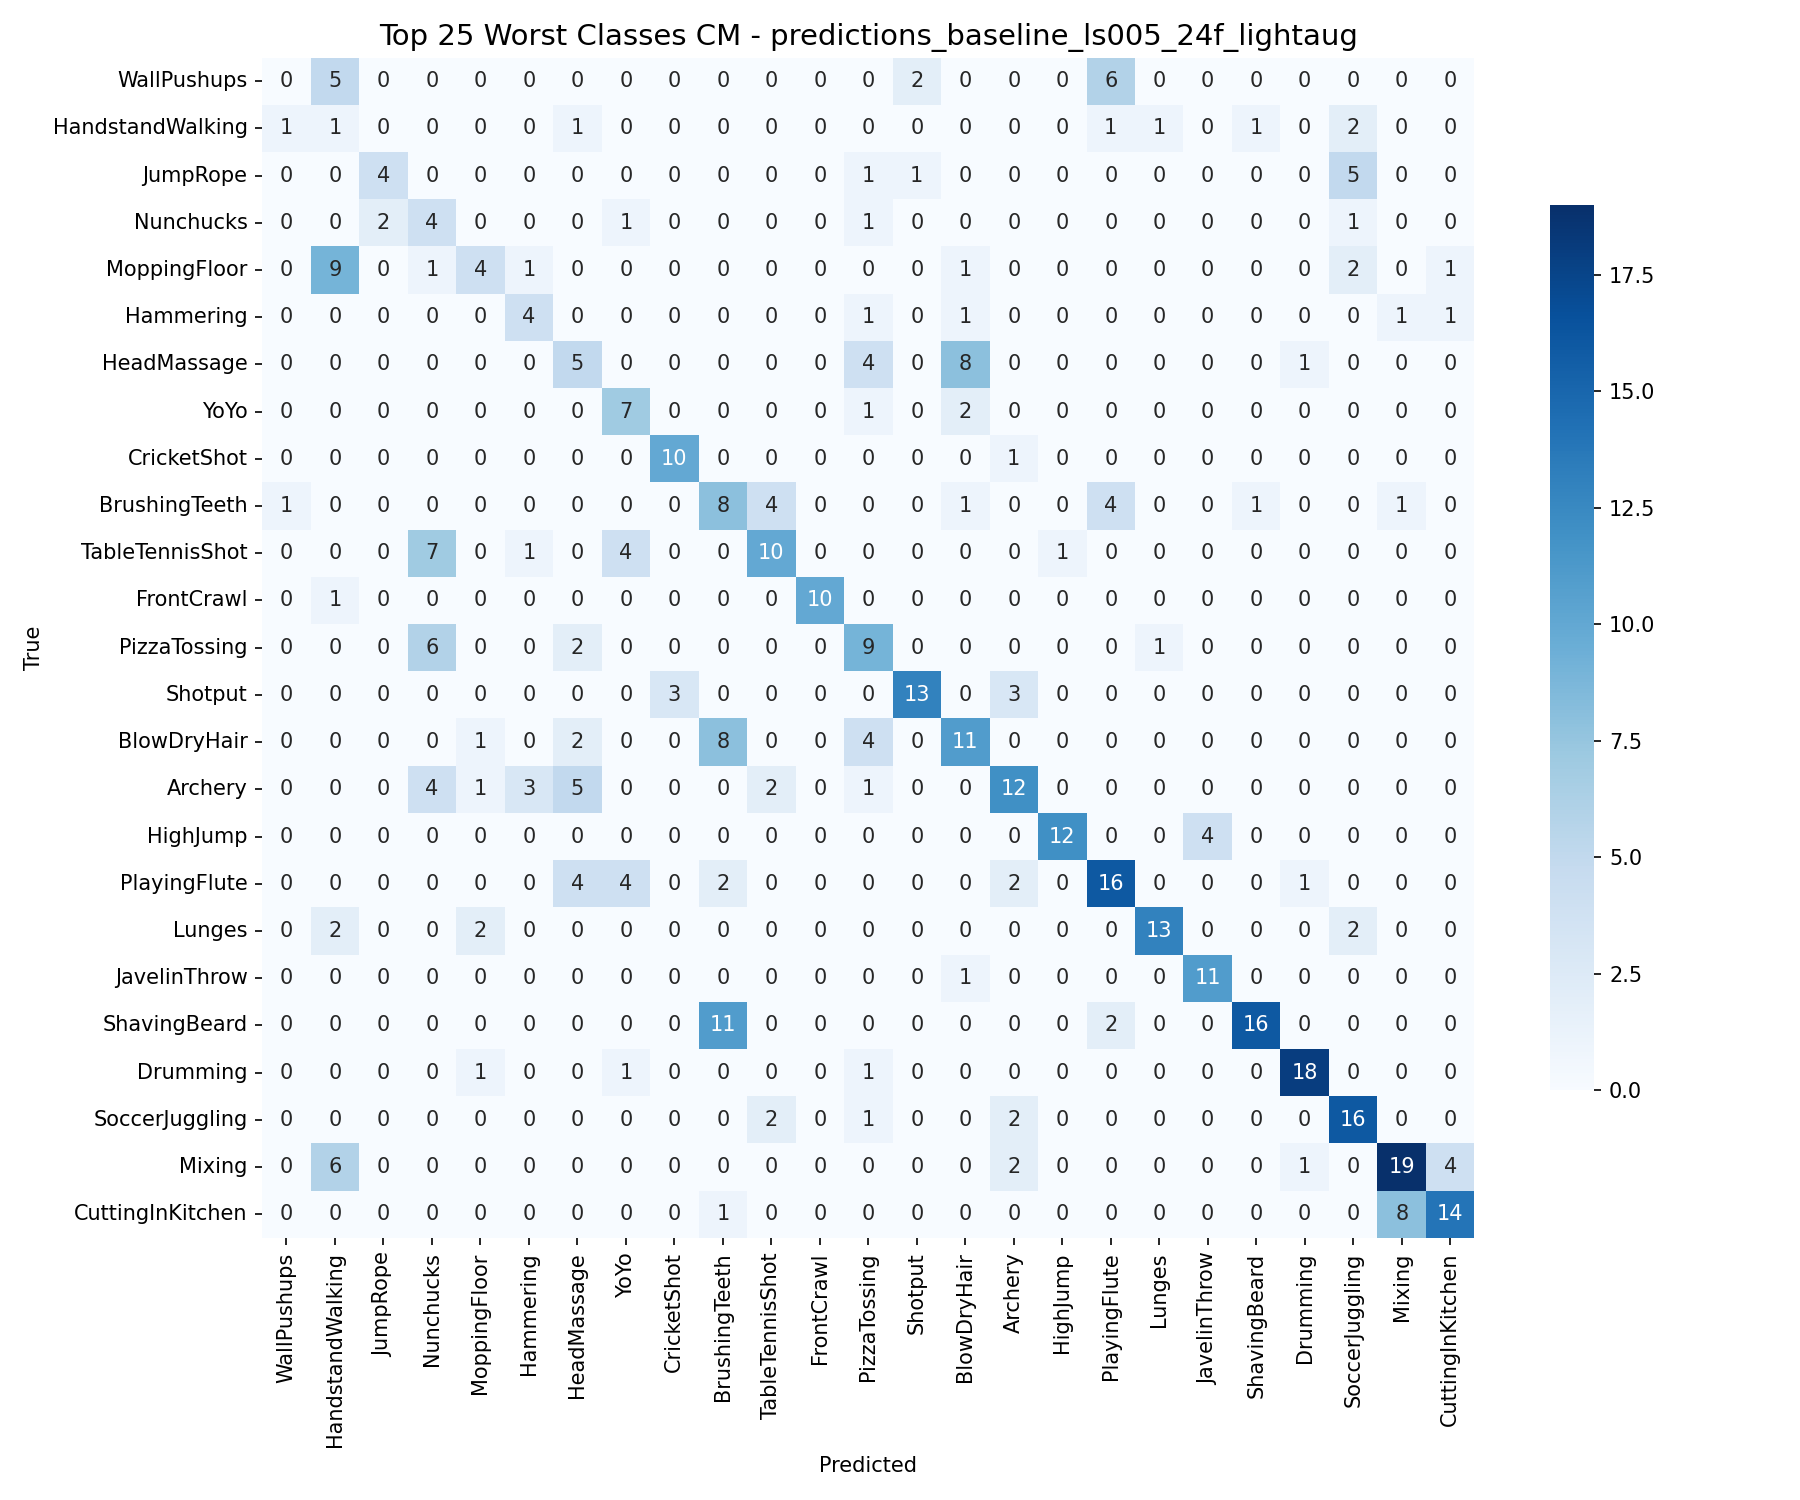
\includegraphics[width=0.85\textwidth]{parts/cap6_risultati/confusion_matrices/predictions_baseline_ls005_24f_lightaug_top25.png}
    \caption{Confusion matrix Top-25 del Baseline: pattern di confusione più diffusi, in particolare tra azioni sportive visivamente simili.}
    \label{fig:cm_baseline}
\end{figure}

\begin{figure}[H]
    \centering
    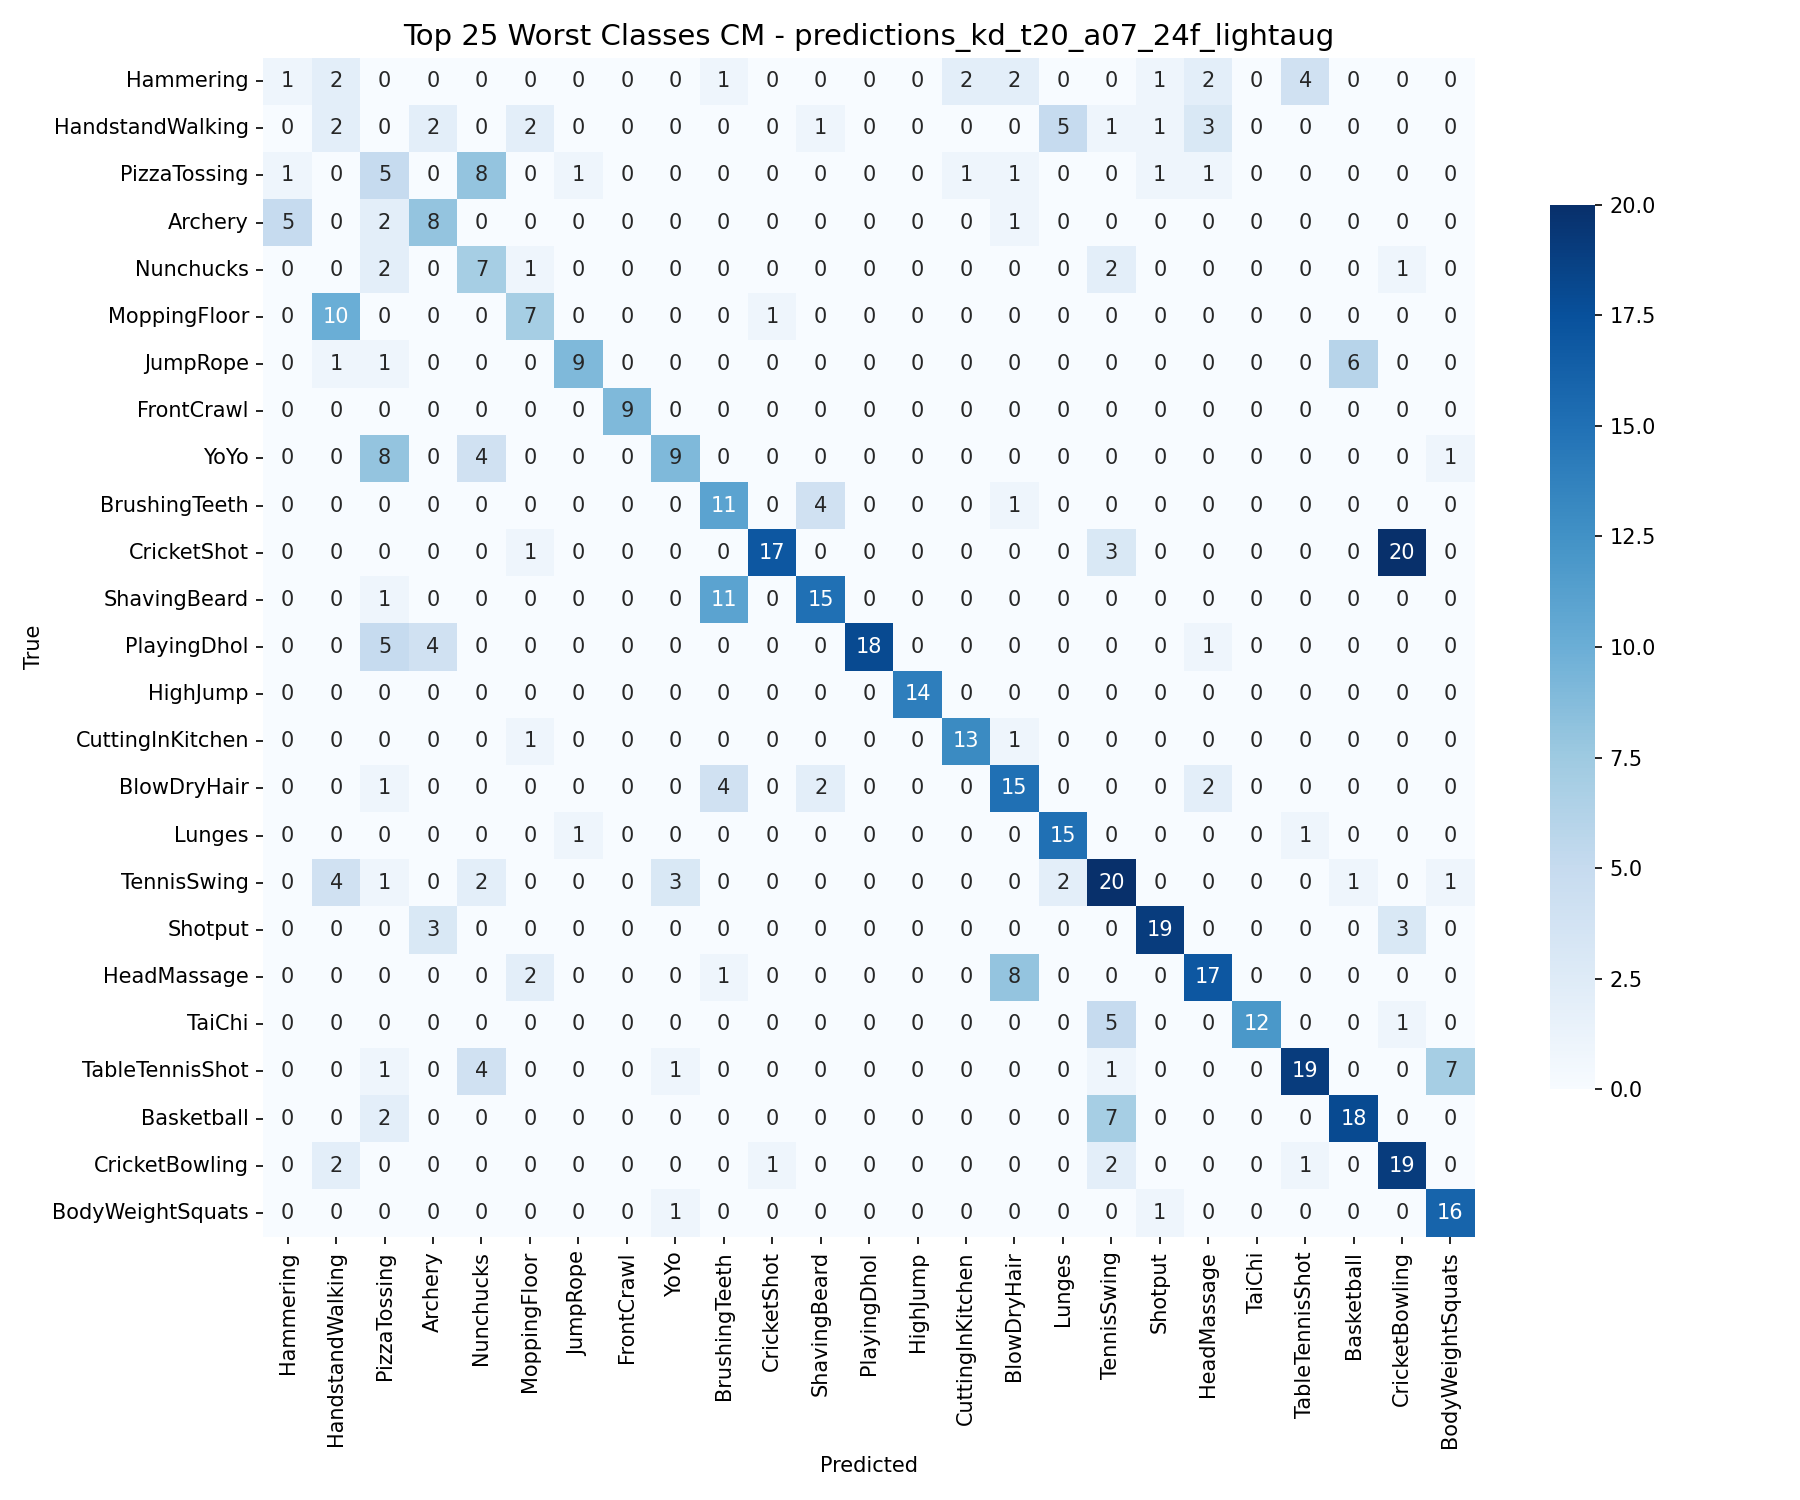
\includegraphics[width=0.85\textwidth]{parts/cap6_risultati/confusion_matrices/predictions_kd_t20_a07_24f_lightaug_top25.png}
    \caption{Confusion matrix Top-25 del migliore Student distillato (KD $T=20$): pattern di errore ridotto rispetto al baseline, evidenziando un trasferimento effettivo della conoscenza discriminativa del teacher.}
    \label{fig:cm_kd_best}
\end{figure}

\section{Riepilogo Quantitativo}

\begin{table}[H]
\centering
\caption{Riepilogo completo di tutti gli esperimenti con split group-aware.}
\label{tab:summary}
\begin{tabular}{lcccc}
\toprule
\textbf{Esperimento} & \textbf{Val Top-1} & \textbf{Test Top-1} & \textbf{Test Top-5} & \textbf{$\Delta$} \\
\midrule
Teacher (ResNet-50)     & 92.36\% & 88.82\% & 98.18\% & upper bound \\
Baseline (MobileNet3D)  & 59.18\% & 59.48\% & 82.77\% & reference \\
\midrule
KD $T=1$, $\alpha=0.7$  & 62.75\% & 62.91\% & 85.59\% & +3.43\% \\
KD $T=5$, $\alpha=0.7$  & 63.12\% & 62.07\% & 87.02\% & +2.59\% \\
KD $T=8$, $\alpha=0.7$  & 64.57\% & 64.31\% & 87.68\% & +4.83\% \\
KD $T=10$, $\alpha=0.7$ & 64.85\% & 64.47\% & 87.44\% & +4.99\% \\
KD $T=20$, $\alpha=0.7$ & 65.18\% & \textbf{65.85\%} & \textbf{87.81\%} & \textbf{+6.37\%} \\
\midrule
AT Simmetrico            & 58.25\% & --- & --- & $-5.93$\% val \\
AT Temporal-Only         & 59.04\% & --- & --- & $-5.14$\% val \\
\midrule
Born-Again Gen 1         & 60.78\% & 60.98\% & --- & $-3.33$\% \\
Born-Again Gen 2         & 61.20\% & 60.43\% & --- & $-3.88$\% \\
Born-Again Gen 3         & 59.98\% & 59.21\% & --- & $-5.10$\% \\
\bottomrule
\end{tabular}
\end{table}
